\documentclass[letterpaper, 10pt, conference]{ieeeconf}
\IEEEoverridecommandlockouts
\overrideIEEEmargins

\usepackage[utf8]{inputenc}
\usepackage[T1]{fontenc}
\usepackage[croatian]{babel}
\usepackage{lmodern}
\usepackage{graphicx}
\usepackage{amsmath,amssymb}
\usepackage{booktabs}
\usepackage{tikz}
\usetikzlibrary{arrows.meta, positioning}

\title{\LARGE \bf ML5 --- Strojno učenje za detekciju anomalija \\[2pt]
\large Machine Learning for Anomaly Detection}

\author{Ime Prezime$^{1}$%
\thanks{$^{1}$Autor je student na Tehničkom fakultetu, Sveučilište u Rijeci,
kolegij Strojno učenje (ML5). {\tt\small ime.prezime@email.com}}%
}

\begin{document}
\maketitle
\thispagestyle{empty}
\pagestyle{empty}

\begin{abstract}
% TASK 9
\end{abstract}

\section{\textbf{UVOD}}
Prijevare kreditnim karticama predstavljaju rastući globalni problem koji financijskim institucijama godišnje uzrokuje gubitke u milijardama dolara. Automatska detekcija prijevarnih transakcija iznimno je zahtjevna zbog ekstremne neuravnoteženosti klasa: u skupu podataka koji se razmatra, svega 0,17\% transakcija jest prijevarno, što odgovara omjeru klasa od otprilike 1:577 \cite{kaggle}. U takvim uvjetima uobičajena mjera točnosti (engl.\ \emph{accuracy}) postaje praktički beznačajna --- klasifikator koji proglasi sve transakcije legitimnima dostiže točnost iznad 99\%, a pritom ne detektira ni jednu prijevaru. Stoga je potrebno koristiti mjere koje su robusne na neuravnoteženost, a sama detekcija anomalija nameće se kao prirodni pristup problemu.

Nenadzirano učenje posebno je prikladno za ovaj problem jer su oznake prijevarnih transakcija u praksi skupe za dobivanje, rijetke i često nepouzdane. Nenadzirani detektori anomalija uče statistički model normalnog ponašanja i označavaju transakcije koje znatno odstupaju od tog modela kao anomalije. Algoritmi se razlikuju po pristupu: metode temeljene na granici odluke, poput One-Class SVM \cite{ocsvm}, opisuju kompaktnu regiju normalne klase u prostoru značajki; metode temeljene na izolaciji, poput Isolation Forest \cite{iforest}, eksploatiraju činjenicu da se anomalije lakše izoliraju od normalnih točaka; metode temeljene na gustoći, poput Local Outlier Factor \cite{lof}, mjere lokalnu gustoću susjedstva svake točke i označavaju one s izrazito nižom gustoćom. Kombinacijom ovih pristupa moguće je pokriti različite manifestacije prijevarnog ponašanja.

Referentni rad koji ovaj rad uzima kao polazište je studija Agyemanga (2024) \cite{agyemang}, koja uspoređuje nekoliko nenadziranih algoritama za detekciju anomalija. Međutim, ta je studija provedena na simuliranom skupu od svega 220 dvodimenzionalnih točaka, što značajno ograničava primjenjivost zaključaka. Autori sami ističu da validacija na stvarnim, visoko-dimenzijskim i neuravnoteženim podacima ostaje otvoren problem. Upravo to ograničenje čini motivaciju za ovaj rad: replicirati eksperimentalni postav na velikom, stvarnom skupu podataka kako bi se provjerilo vrijede li zaključci iz simulacijske studije i u realnom scenariju.

Cilj ovog rada je primijeniti identičan skup algoritama i hiperparametara na stvarni skup podataka o transakcijama kreditnim karticama \cite{kaggle} koji broji 284\,807 transakcija i sadrži 30 numeričkih značajki dobivenih PCA transformacijom. Kao prag za otkrivanje anomalija uvodi se \emph{label-free} MAD (engl.\ \emph{Median Absolute Deviation}) pristup koji ne koristi oznake klasa ni procjenu stvarne stope prijevara, čime se simulira realan scenarij bez nadziranog signala. Provedena je i analiza skalabilnosti algoritama prelaskom po veličinama uzorka od 30\,000 do 230\,000 transakcija. Primarna mjera kvalitete je površina ispod ROC krivulje (ROC-AUC), koja ocjenjuje sposobnost rangiranja prijevarnih transakcija neovisno o odabranom pragu. Glavni nalaz rada jest da jaki modeli odlično rangiraju prijevarne transakcije (visoki ROC-AUC), no precizno pragovanje bez oznaka klasa ostaje ključno usko grlo pri primjeni u praksi.

\section{\textbf{METODOLOGIJA}}
\subsection{Pregled modela}

Eksperiment obuhvaća šest nenadziranih detektora anomalija i jedan nadzirani baseline, sažeto prikazane u Tablici~\ref{tab:lineup}.
\textbf{One-Class SVM} \cite{ocsvm} uči kompaktnu RBF granicu oko normalnih uzoraka u prostoru značajki; sve točke izvan te granice označava kao anomalije.
\textbf{One-Class SVM (SGD)} je linearna SGD aproksimacija iste ideje koja se bolje skalira na veće skupove podataka.
\textbf{Isolation Forest} \cite{iforest} nasumično izolira točke rekurzivnim podjelama; anomalije se izoliraju s manjim brojem rezova jer su u rijetkim regijama prostora.
\textbf{Local Outlier Factor (LOF)} \cite{lof} mjeri lokalnu gustoću susjedstva svake točke i označava one čija je gustoća bitno niža od gustoće susjeda.
\textbf{Robust Covariance / Elliptic Envelope} \cite{mcd} procjenjuje Gaussovu elipsu na temelju minimalne kovarijarijske determinante (MCD) i mjeri Mahalanobisovu udaljenost svake točke od središta.
\textbf{Autoencoder} \cite{pytorch} je neuronska mreža arhitekture 30→20→14→20→30 trenirana isključivo na normalnim uzorcima (PyTorch, GPU); anomalije uzrokuju veću rekonstrukcijsku pogrešku (MSE). Budući da jedino Autoencoder koristi GPU, njegovo izvođenje nije izravno usporedivo s ostalima po trajanju; ROC-AUC ostaje pošten zajednički nazivnik.
\textbf{Logistička regresija} \cite{sklearn} jedini je nadzirani model i služi kao gornja referentna granica (baseline): trenira se na 70\% stratificiranog poduzorka i vrednuje na preostalih 30\%, koristeći uravnotežene težine klasa.
Cjelokupni postav pipeline-a prikazan je na Slici~\ref{fig:pipeline}.

\begin{table}[t]
\caption{Skup algoritama i ključni hiperparametri. Prvih šest su nenadzirani; Logistička regresija je nadzirani baseline.}
\label{tab:lineup}
\centering
\begin{tabular}{@{}lll@{}}
\toprule
Model & Hiperparametri & Ocjena anomalije \\
\midrule
One-Class SVM        & RBF, $\gamma{=}0.1$, $\nu{=}0.05$        & $-$\,decision\_function \\
One-Class SVM (SGD)  & $\nu{=}0.05$, max\_iter${=}1000$         & $-$\,decision\_function \\
Isolation Forest     & $n{=}100$, contamination${=}$auto       & $-$\,decision\_function \\
Local Outlier Factor & $k{=}20$, novelty${=}$False             & $-$\,neg.\ outlier factor \\
Robust Covariance    & contamination${=}0.1$                   & $-$\,decision\_function \\
Autoencoder (GPU)    & $(20,14)$, 30 ep., bs${=}2048$          & rekonstr.\ MSE \\
Logistic Regression  & class\_weight${=}$balanced              & predict\_proba \\
\bottomrule
\end{tabular}
\end{table}

\subsection{Ujednačeni anomaly score}

Da bi se ROC-AUC mogao izračunati na jednak način za sve modele, svi detektori svedeni su na jedinstvenu konvenciju \emph{``veće = anomalnije''}.
Scikit-learn modeli koji izlažu metodu \texttt{decision\_function} vraćaju vrijednosti kod kojih \emph{niži} rezultat znači anomaliju; stoga se te vrijednosti negiraju.
Kod LOF-a u načinu rada \texttt{fit\_predict} (bez \texttt{novelty=True}) direktno se negira atribut \texttt{negative\_outlier\_factor\_}.
Autoencoder izravno vraća rekonstrukcijsku MSE pogrešku, koja je već u konvenciji ``veće = anomalnije''.
Ova konvencija predznaka je nužna: bez negiranja, ROC-AUC kod relevantnih modela bio bi ispod 0,5, tj.\ invertirani ranking.

\subsection{Label-free MAD prag}

Za pretvaranje kontinuiranih anomaly scoreova u binarne predikcije koristi se robusni modificirani z-score temeljen na medijalnoj apsolutnoj devijaciji (MAD) \cite{mad}. Svaka ocjena $s_i$ se standardizira prema:

\begin{equation}
z_i = \frac{s_i - \mathrm{med}(s)}{1.4826 \cdot \mathrm{MAD}(s)}, \qquad
\text{anomalija} \iff z_i > k, \quad k = 3.0
\label{eq:mad}
\end{equation}

Faktor 1.4826 čini MAD konzistentnim procjeniteljem standardne devijacije za normalnu distribuciju. Prag $k = 3.0$ odabran je kao standardna vrijednost iz literature \cite{mad}. Ova metoda je u potpunosti \emph{label-free}: udio transakcija označenih kao anomalije (``implied contamination'') određen je isključivo distribucijom scoreova, a stvarna stopa prijevara ne ulazi u detekciju --- koristi se samo za vrednovanje na kraju.

\subsection{Mjere vrednovanja}

Primarna mjera je \textbf{ROC-AUC} (površina ispod ROC krivulje), izračunata na kontinuiranim anomaly scoreovima. ROC-AUC je neovisan o izboru praga, mjeri sposobnost rangiranja prijevarnih transakcija ispred legitimnih i robustan je na neuravnoteženost klasa --- sve osobine poželjne u ovom scenariju. Dodatno se izvještava pet mjera na binarnim predikcijama (dobivenim MAD pragom iz jednadžbe~\eqref{eq:mad}): točnost (Accuracy), preciznost (Precision), odziv (Recall), F1-mjera i koeficijent determinacije $R^2$. Napominje se da ``implied contamination'' (udio označenih točaka) tipično premašuje stvarnu stopu prijevara od 0,17\% jer MAD prag nije kalibriran na stvarnu stopu --- što je i namjeravano ponašanje u scenariju bez oznaka.

\begin{figure}[t]
\centering
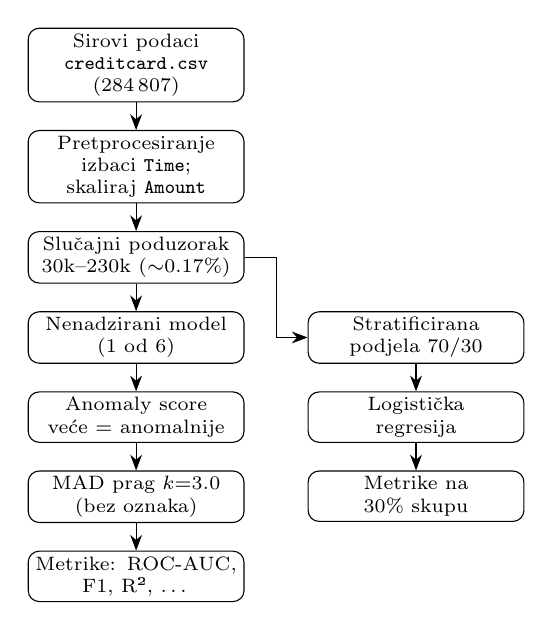
\begin{tikzpicture}[
  font=\scriptsize, node distance=3.5mm,
  box/.style={draw, rounded corners, align=center, inner sep=2pt,
              text width=2.6cm, minimum height=6mm},
  arr/.style={-{Stealth[length=2mm]}}]
\node[box] (data) {Sirovi podaci\\ \texttt{creditcard.csv}\\ (284\,807)};
\node[box, below=of data] (prep) {Pretprocesiranje\\ izbaci \texttt{Time};\\ skaliraj \texttt{Amount}};
\node[box, below=of prep] (samp) {Slučajni poduzorak\\ 30k--230k ($\sim$0.17\%)};
\node[box, below=of samp] (model) {Nenadzirani model\\ (1 od 6)};
\node[box, below=of model] (score) {Anomaly score\\ veće $=$ anomalnije};
\node[box, below=of score] (mad) {MAD prag $k{=}3.0$\\ (bez oznaka)};
\node[box, below=of mad] (met) {Metrike: ROC-AUC,\\ F1, R², \dots};
\node[box, right=8mm of model] (split) {Stratificirana\\ podjela 70/30};
\node[box, below=of split] (lr) {Logistička\\ regresija};
\node[box, below=of lr] (met2) {Metrike na\\ 30\% skupu};
\draw[arr] (data) -- (prep);
\draw[arr] (prep) -- (samp);
\draw[arr] (samp) -- (model);
\draw[arr] (model) -- (score);
\draw[arr] (score) -- (mad);
\draw[arr] (mad) -- (met);
\draw[arr] (samp.east) -- ++(0.4,0) |- (split.west);
\draw[arr] (split) -- (lr);
\draw[arr] (lr) -- (met2);
\end{tikzpicture}
\caption{Tok podataka. Nenadzirani modeli (lijevo) ocjenjuju se na cijelom poduzorku bez podjele; nadzirani baseline (desno) uči na 70\% i vrednuje se na 30\%.}
\label{fig:pipeline}
\end{figure}

\section{\textbf{STUDIJA SLUČAJA}}
% TASK 6
\subsection{Skup podataka}
\subsection{Vrednovanje}

\section{\textbf{REZULTATI I RASPRAVA}}
% TASK 7 (tables + figures) and TASK 8 (discussion)

\section{\textbf{ZAKLJUČAK}}
% TASK 9

\begin{thebibliography}{99}
\bibitem{agyemang} E. F. Agyemang, ``Anomaly detection using unsupervised machine learning algorithms: A simulation study,'' \emph{Scientific African}, vol.~26, e02386, 2024.
\bibitem{kaggle} Machine Learning Group, Université Libre de Bruxelles, ``Credit Card Fraud Detection,'' Kaggle, 2018. [Online]. Available: \texttt{https://www.kaggle.com/mlg-ulb/creditcardfraud}
\bibitem{sklearn} F. Pedregosa \emph{et al.}, ``Scikit-learn: Machine learning in Python,'' \emph{J. Mach. Learn. Res.}, vol.~12, pp.~2825--2830, 2011.
\bibitem{ocsvm} B. Schölkopf, J. C. Platt, J. Shawe-Taylor, A. J. Smola, and R. C. Williamson, ``Estimating the support of a high-dimensional distribution,'' \emph{Neural Comput.}, vol.~13, no.~7, pp.~1443--1471, 2001.
\bibitem{iforest} F. T. Liu, K. M. Ting, and Z.-H. Zhou, ``Isolation forest,'' in \emph{Proc. 8th IEEE Int. Conf. Data Mining (ICDM)}, 2008, pp.~413--422.
\bibitem{lof} M. M. Breunig, H.-P. Kriegel, R. T. Ng, and J. Sander, ``LOF: Identifying density-based local outliers,'' in \emph{Proc. ACM SIGMOD Int. Conf. Management of Data}, 2000, pp.~93--104.
\bibitem{mcd} P. J. Rousseeuw and K. Van Driessen, ``A fast algorithm for the minimum covariance determinant estimator,'' \emph{Technometrics}, vol.~41, no.~3, pp.~212--223, 1999.
\bibitem{mad} B. Iglewicz and D. C. Hoaglin, \emph{How to Detect and Handle Outliers}. Milwaukee, WI: ASQC Quality Press, 1993.
\bibitem{pytorch} A. Paszke \emph{et al.}, ``PyTorch: An imperative style, high-performance deep learning library,'' in \emph{Adv. Neural Inf. Process. Syst. 32 (NeurIPS)}, 2019, pp.~8024--8035.
\end{thebibliography}

\end{document}
